\documentclass{beamer}

\usepackage{etex}
\usepackage[utf8]{inputenc}
\usepackage[T1]{fontenc}
\usepackage[frenchb]{babel}
\usepackage{hyperref}
\usepackage{graphicx}
\usepackage{animate}
\usepackage{tikz}
\usepackage{pgfplots}

\DeclareUnicodeCharacter{00A0}{ }

\usetheme{Berkeley}

\title{Le problème SAT}
\subtitle{TIPE math}
\author{Luc Chabassier}
\institute{Lycée Pierre de Fermat}

\setbeamertemplate{itemize item}[ball]
\setbeamertemplate{itemize subitem}[triangle]
\setbeamertemplate{itemize subsubitem}[circle]
\setbeamertemplate{blocks}[rounded][shadow=true]

\begin{document}
\begin{frame}
    \maketitle
\end{frame}

\section{SAT}
\subsection{Présentation}
% Frame 1 : présentation du problème SAT
\begin{frame}
    \frametitle{Présentation générale}
    \begin{block}{Définition}
        Problème de décision : recherche d'une valuation évaluant à vrai pour une formule booléenne.
    \end{block}

    \begin{exampleblock}{Exemple}
        \begin{itemize}
            \item UNSAT : $(x_0\vee x_1) \wedge (\neg x_0\vee x_1) \wedge (x_0\vee\neg x_1) \wedge (\neg x_0\vee\neg x_1)$
            \item SAT : ${\color{green}{\color{blue}x_0}\wedge\neg{\color{red}({\color{blue}x_0}\wedge\neg{\color{green}({\color{blue}x_1}\wedge\neg{\color{red}({\color{blue}x_1}\wedge {\color{orange}x_2})})})}}$
        \end{itemize}
    \end{exampleblock}
    \begin{exampleblock}{Applications}
        \begin{itemize}
            \item En cryptographie.
            \item En résolution de dépendances.
            \item En biologie.
        \end{itemize}
    \end{exampleblock}
    \begin{alertblock}{NP-Complet : théorème de Cook 1971}
    \end{alertblock}
\end{frame}

\subsection{k-SAT}
% Frame 2 : cas du k-SAT
\begin{frame}
    \frametitle{Cas particulier du k-SAT}
    \begin{exampleblock}{Forme normale conjonctive}
        $(h\vee\neg b) \wedge (e\vee\neg h\vee\neg c) \wedge (\neg g\vee\neg d\vee\neg c) \wedge (a\vee\neg h\vee d) \wedge (a\vee\neg d\vee\neg e\vee g)$
    \end{exampleblock}
    \begin{block}{NP-Complet}
        \[ \begin{array}{cl}
                & x_0 \wedge \neg(x_0 \wedge \neg(x_1 \wedge \neg (x_1 \wedge x_2))) \\
                \equiv & x_0 \wedge (\neg x_0 \vee (x_1 \wedge (\neg x_1 \vee \neg x_2))) \\
                \equiv & x_0 \wedge (\neg x_0 \vee a) \wedge (\neg x_1 \vee \neg x_2 \vee \neg a) \\
           \end{array}
        \]
    \end{block}
    \begin{alertblock}{Plus fort}
        Le 3-SAT est NP-complet
    \end{alertblock}
\end{frame}

\subsection{2-SAT}
% Frame 3 : cas du 2-SAT
% théorème de Ladner pour l'existence de problème ni P ni NP-complet
% théorème de dichotomie de Schaefer
\begin{frame}
    \frametitle{Cas particulier du 2-SAT}
    \begin{block}{Résolvable en temps linéaire}
        \[ x_1 \vee x_2 \equiv (\neg x_1 \Rightarrow x_2) \wedge (\neg x_2 \Rightarrow x_1) \]
        % TODO exemple de graphe
    \end{block}
    \begin{exampleblock}{Remarque}
        Effet de palier entre 2-SAT et 3-SAT.
    \end{exampleblock}
\end{frame}

\section{Algorithme}
\subsection{CDCL}
% Frame 4 : algorithme CDCL
\begin{frame}
    \frametitle{Algorithme CDCL}
    \begin{center}
        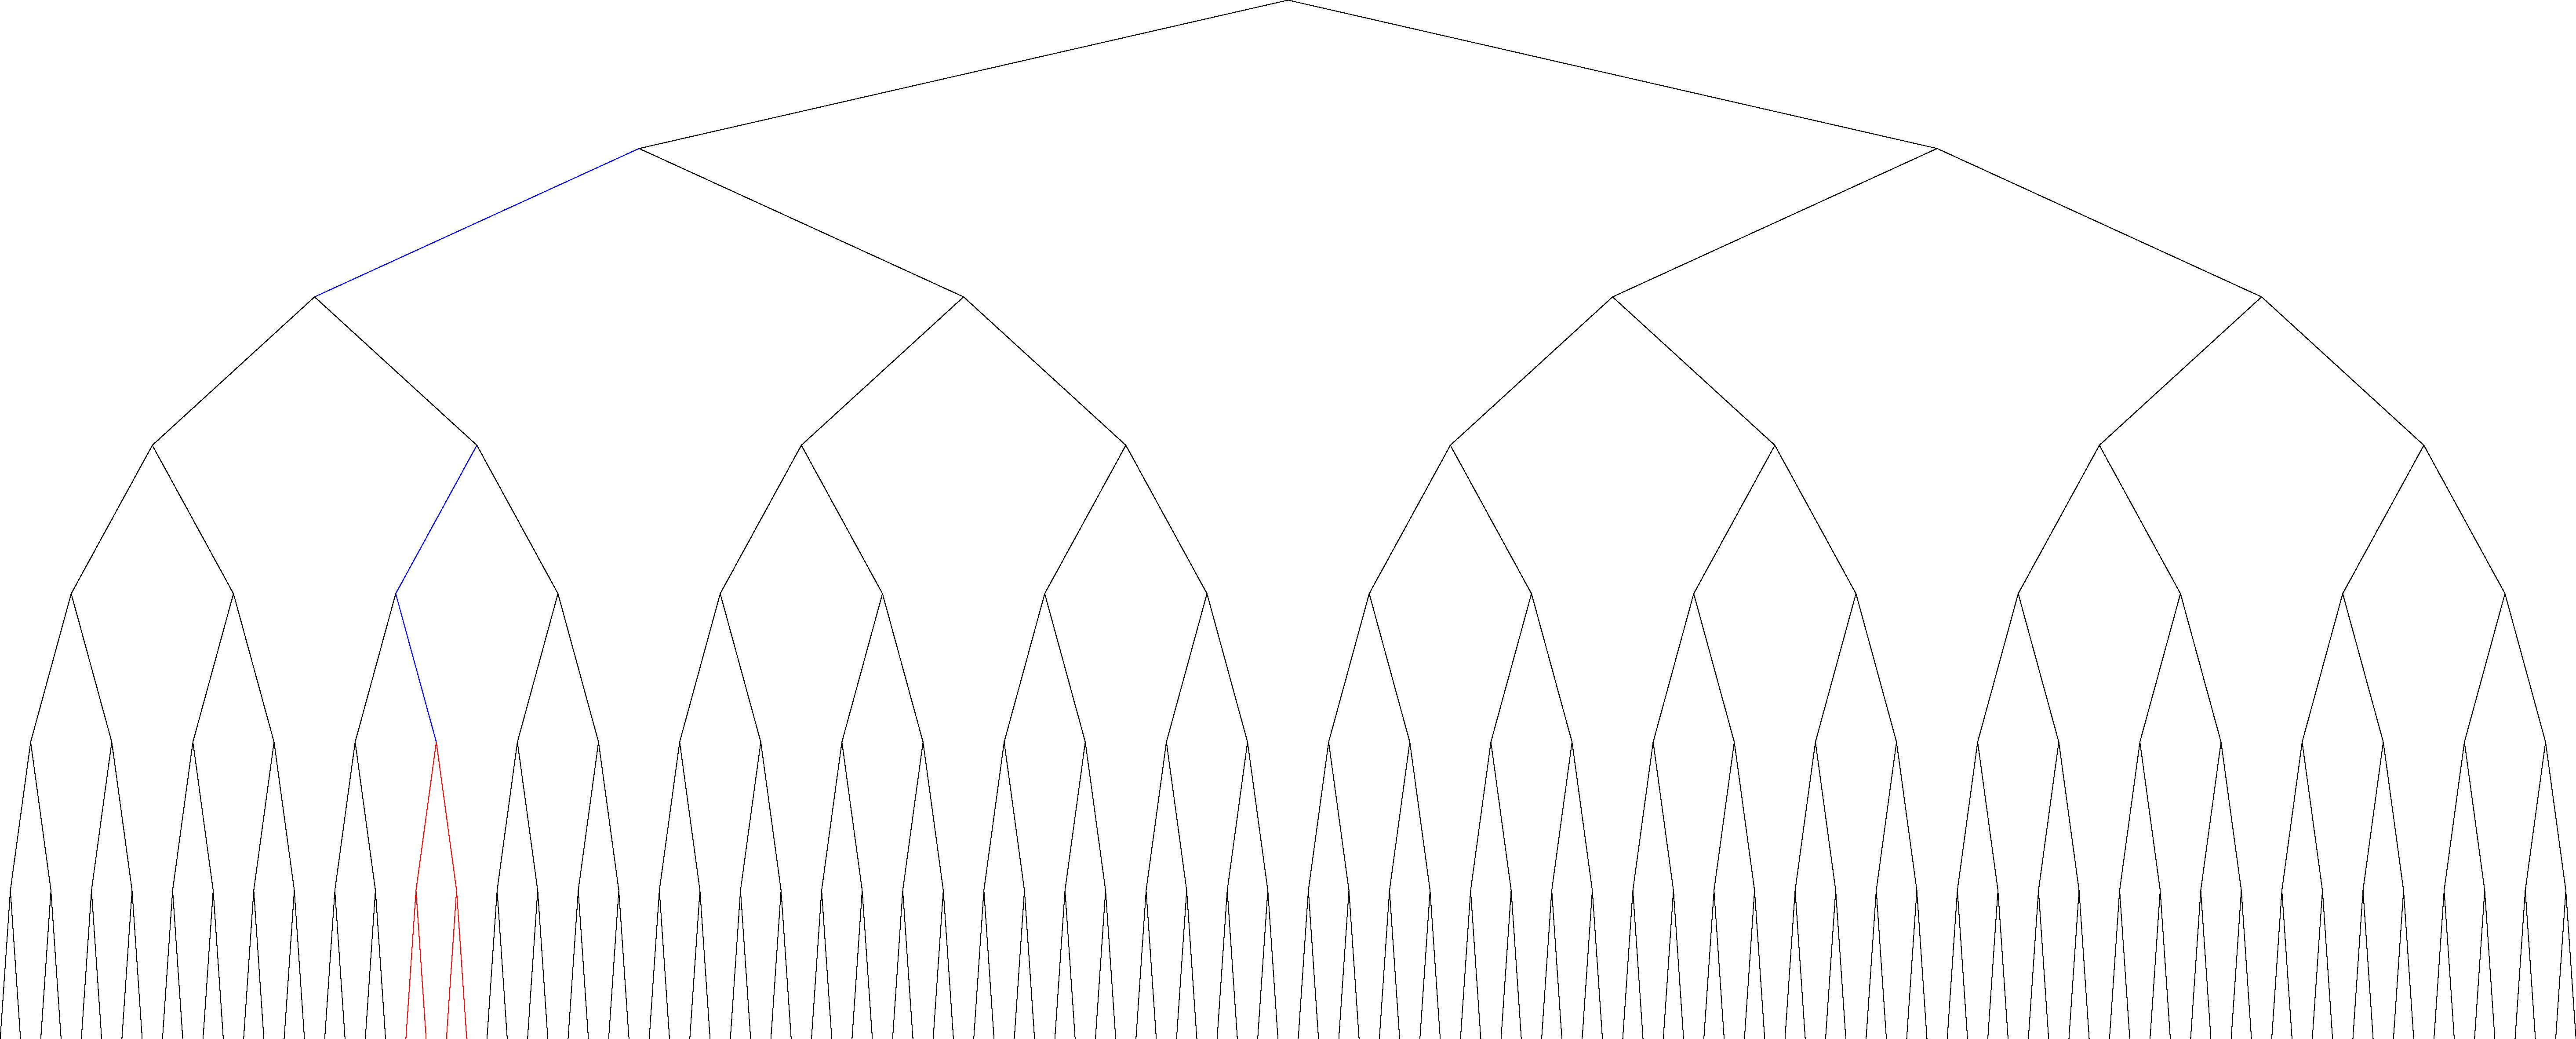
\includegraphics[width=0.8\linewidth]{../reso/error.pdf} \\
        \vspace{1em}
        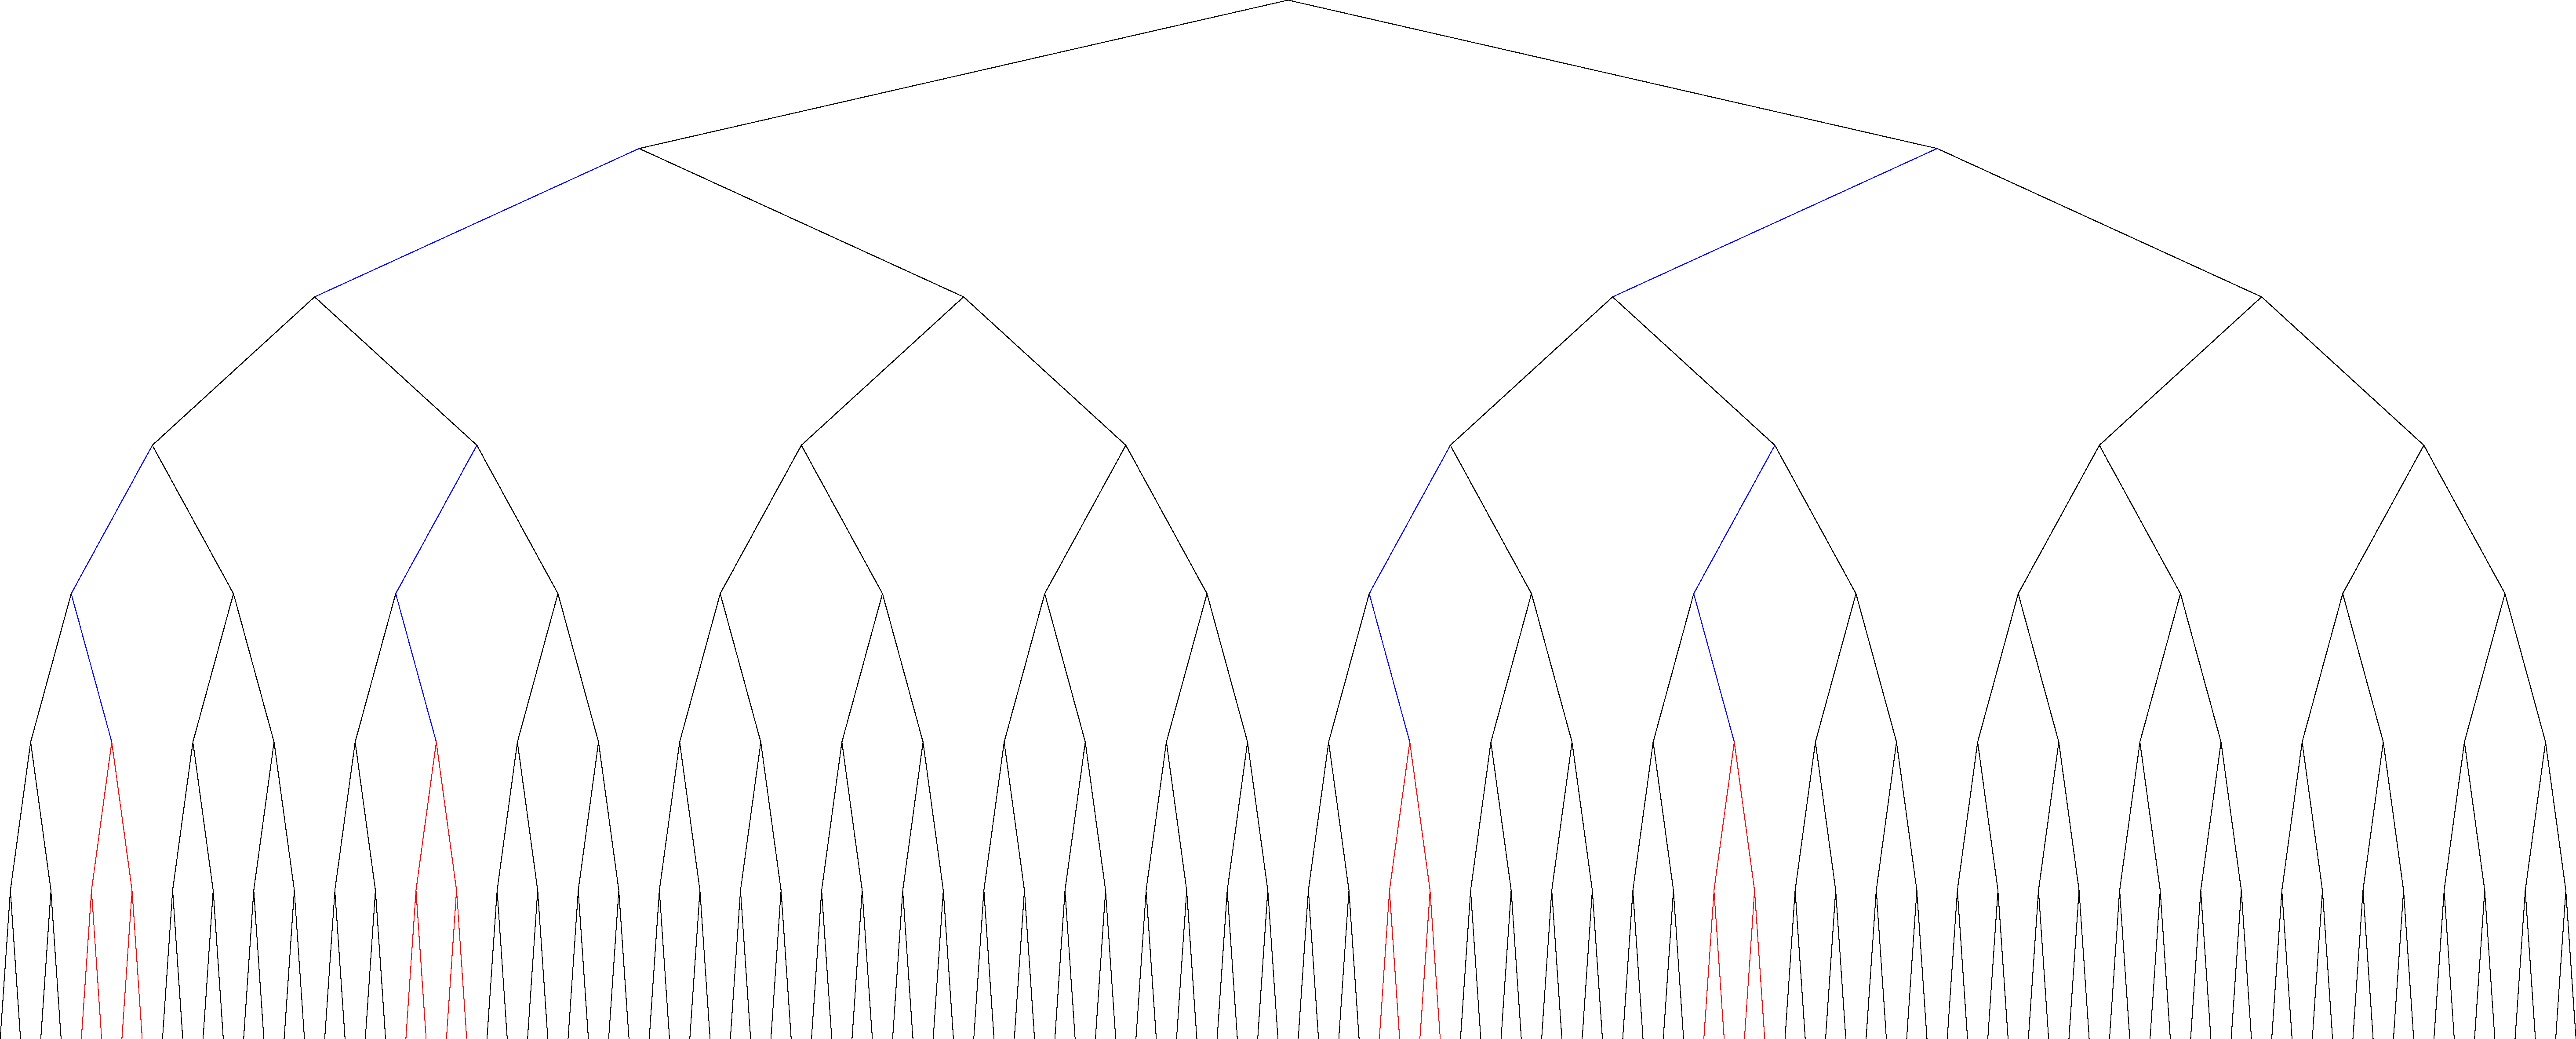
\includegraphics[width=0.8\linewidth]{../reso/eliminated.pdf}
    \end{center}
\end{frame}

\subsection{Redémarrages}
% Frame 5 : redémarrages
\begin{frame}
    \frametitle{Redémarrages}
    \begin{block}{Gain de temps sur des instances SAT.}
        Stratégie de redémarrage : $(t_n)_{n\in\mathbb{N}}\in(\mathbb{N}^*)^\mathbb{N}$
    \end{block}
    \begin{exampleblock}{Stratégies usuelles}
        \begin{itemize}
            \item Stratégie fixée : $t_n$ constant.
            \item Stratégie géométrique : $t_n$ géométrique.
            \item Stratégie de Luby : multiple de la suite de luby.
                \[ \forall i\in\mathbb{N}^*, t_i = \left\{\begin{array}{cl}
                                                           2^{k-1} & \text{if } i = 2^k-1 \\
                                                           t_{i-2^{k-1}+1} & \text{if } 2^{k-1}\leq i<2^k-1
                                                         \end{array}\right.\]
            \item \emph{Nested Restart Strategy} : version simplifiée de la stratégie de Luby.
        \end{itemize}
    \end{exampleblock}
\end{frame}

\subsection{Heuristiques}
% Frame 6 : Heuristiques dans le choix de la variable
\begin{frame}
    \frametitle{Heuristiques dans le choix de la variable}
    \begin{block}{Objectif}
        Favoriser l'apparition des conflits.
    \end{block}
    \begin{exampleblock}{Heuristiques usuelles}
        \begin{itemize}
            \item \emph{Dynamic Largest Individual Sum (DLIS)}
            \item \emph{Jeroslow-Wang (JW)} et \emph{Maximum Ocurrence of clauses of Minimum size (MOM)}
            \item \emph{Variable State Independant Decaying Sum (VSIDS)}
        \end{itemize}
    \end{exampleblock}
    \begin{alertblock}{Limites}
        Structures paresseuses.
    \end{alertblock}
\end{frame}

\section{HIPP}
\subsection{Présentation}
% Frame 7 : le problème HIPP
\begin{frame}
    \frametitle{Le problème HIPP}
    \begin{block}{Génome somme d'haplotypes}
            \[ \left(\begin{array}{c} 1 \\ 1 \\ 0 \end{array}\right) \bigoplus \left(\begin{array}{c} 1 \\ 0 \\ 0\end{array}\right) =
                \left(\begin{array}{c} 1 \\ 2 \\ 0 \end{array}\right) \]
    \end{block}
    \begin{block}{Objectif}
        Minimisation de l'ensemble d'haplotypes pour une population.
    \end{block}
    La population
    \[\begin{array}{c} \{(0,0,0,1),(1,0,0,1),(0,1,0,1), \\ (2,0,0,1),(0,2,0,1),(2,2,0,1)\}\end{array} \]
    peut se déduire des haplotypes
    \[\{(0,0,0,1),(1,0,0,1),(0,1,0,1)\}\]
\end{frame}

\subsection{SAT}
% Frame 8 : Algorithme utilisant le SAT
\begin{frame}
    \frametitle{Utilisation du k-SAT pour résoudre le problème HIPP}
    \begin{itemize}
        \item $r$ haplotypes, $n$ génomes de taille $m$ : $(g_i(j))$.
        \item Haplotypes : $h_i(j)$ pour $1\leq i\leq r$, $1\leq j\leq m$
        \item Sélection : $s^a_i(j)$ et $s^b_i(j)$ pour $1\leq i\leq n$, $1\leq j\leq r$
    \end{itemize}
    \[ \bigwedge_{i=1}^n\left[\bigwedge_{j=1}^r s^a_i(j) \vee \bigwedge_{j=1}^r s^b_i(j)\right] \]
    Pour un génome $i$ et une position $j$ : \begin{itemize}
        \item $g_i(j) = 0$ : $\bigwedge_{k=1}^r (\neg s^a_i(k)\vee \neg h_k(j)) \wedge (\neg s^b_i(k)\vee \neg h_k(j))$
        \item $g_i(j) = 1$ : $\bigwedge_{k=1}^r (\neg s^a_i(k)\vee h_k(j)) \wedge (\neg s^b_i(k)\vee h_k(j))$
        \item $g_i(j) = 2$ : $(b_1\vee b_2) \wedge (\neg b_1\vee \neg b_2)$
            \[\bigwedge_{k=1}^r \left(\begin{array}{cl}
                        & (\neg s^a_i(j)\vee b_1 \vee h_k(j)) \\
                 \wedge & (\neg s^a_i(j)\vee \neg b_1\vee \neg h_k(j)) \\
                 \wedge & (\neg s^b_i(j)\vee b_2 \vee h_k(j)) \\
                 \wedge & (\neg s^b_i(j)\vee \neg b_2 \vee \neg h_k(j))
            \end{array}\right)\]
    \end{itemize}
\end{frame}

\subsection{Optimisations}
% Frame 9 : Améliorations de l'algorithme
\begin{frame}
    \frametitle{Spécialisations de l'algorithme SAT}
    \begin{block}{Support du XOR}
        \[ \bigwedge_{i=1}^n\left[\bigoplus_{j=1}^r s^a_i(j) \vee \bigoplus_{j=1}^r s^b_i(j)\right] \]
        \[ (b_1 \vee b_2) \wedge (\neg b_1 \vee \neg b_2) \equiv b_1\oplus b_2 \]
    \end{block}
\end{frame}
\end{document}

